%!TEX root = ../montravail.tex

\chapter{Background}
%\addcontentsline{toc}{chapter}{Grundlagen}
\lhead[ \leftmark   ]{\textbf{Background}}

%erstes Unterkapitel
\section{Human brain and languages}

\textcolor[rgb]{1,0,0}{Lots of studies have tried to teach limited forms of human language to other great apes. Gorillas and chimpanzees have been able to pick up and communicate through symbols and sign languages and even through a limited form of combinations of the
human protolanguage\\\\
possibilities to learn new languages, dolmetchen �bersetzen...\\\\
sens for communoiation}

%n�chstes unterkapitel ebene 2
\subsection{Broca?s area}
Hier schreiben

%unterkapitel Ebene 3 nicht im Inhaltsverzeichnis aufgef�hrt! 
\subsubsection{Dritte �berschrift}
\textit{hier kann Kursiv geschrieben werden}

%zweites Unterkapitel
\section{Erste �berschrift}

%n�chstes unterkapitel ebene 2
\subsection{Zweite �berschrift}

%Abbildungsbeispiel
%Abbildungsquelle immer! angeben es sei den selber gemacht!!!!
Text....(siehe Abb. 1.1)

\begin{figure}[!ht]
	%mitte der Seite
	\centering
		%[nat�rliche Breite in Pixeln, nat�rliche H�he in Pixeln, Abh�ngigkeit von der Textbreite]
		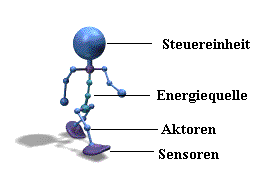
\includegraphics[natwidth=1200pt, natheight=349pt, width=0.4\textwidth]{grafiken/Robotpeintre.PNG}
	\caption[Aufbau allgemein]{Aufbau und Komponenten von Robotern}
	\label{fig:Aufbau und Komponenten von Robotern}
\end{figure}

%unterkapitel Ebene 3 nicht im Inhaltsverzeichnis aufgef�hrt!
\subsubsection{Dritte �berschrift}

%Aufz�hlung
\begin{itemize}
	\item Die Bewegungsform der Achsen
	\item Anzahl und Anordnung der Achsen
	\item Die Formen des Arbeitsraums
\end{itemize}
    
... Arm zu strecken. (Vgl.\cite{112}) 
%n�chstes unterkapitel ebene 2
\subsection{Zweite �berschrift}
%unterkapitel Ebene 3 nicht im Inhaltsverzeichnis aufgef�hrt!
\subsubsection{Dritte �berschrift}
Hier Text einf�gen\index{einf�gen}

%� ohne weiterf�hrung des Wortes
Roboterfu\ss \ befindet

homogene\\ 4 x 4  Matrix:

\begin{equation} 
T = \begin{pmatrix}
     Ax&Ay&Az&0\\Bx&By&Bz&0\\Cx&Cy&Cz&0\\Px&Py&Pz&1
     \end{pmatrix}
\end{equation}


\begin{equation}(\theta, d, a, \alpha)\end{equation}
 
verschiedene Matrizen:

\begin{equation}
T=\begin{pmatrix}\cos\theta & -\sin\theta \cos\alpha & \sin\theta \sin\alpha & \arccos\theta\\ \sin\theta & \cos\theta \cos\alpha & -\cos\theta \sin\alpha & \arcsin\theta\\ 0 & \sin\alpha & \cos\alpha & d\\ 0 & 0 & 0 & 1\end{pmatrix}
\end{equation}

\begin{equation}
^{n - 1}T_n
  = \begin{pmatrix}
    \cos\theta_n & -\sin\theta_n \cos\alpha_n & \sin\theta_n \sin\alpha_n & a_n \cos\theta_n \\
    \sin\theta_n & \cos\theta_n \cos\alpha_n & -\cos\theta_n \sin\alpha_n & a_n \sin\theta_n \\
    0 & \sin\alpha_n & \cos\alpha_n & d_n \\
    0 & 0 & 0 & 1
  \end{pmatrix}.
\end{equation}


\begin{equation}
T=T_1T_2T_3T_4T_5T_{tcp}
\end{equation}


%Beispiel f�r eine Tabelle
Text...(Siehe Tab. 1.1)
\\\\
\textbf{Titel:}\\%Der Titel bei Tabellen muss immer �ber der Tabelle stehen Statuten FH-Koeln! bei Abbildungen drunter! 
\begin{table}[ht]
\centering
\caption[Titel]{Titel}	
	 \begin{tabular}{|c|p{11cm}|}
			\hline
			\rowcolor{sourcegray}
			\textbf{�berschrift 1} & \textbf{�berschrift 2}\\
			\hline
			Text & Text \newline 
						 Text\\
			\hline
			Text & Text \newline 
						 Text\\
			\hline
		\end{tabular}
	\vspace{1.0em}
	%\caption[Mobilit�tsgrade]{Gliederung der Mobilit�tsgrade}
	\label{tab:Titel}
\end{table}

\newpage
%Beispiel f�r zwei Bilder nebeneinander
\begin{figure}[!ht]
\centering 
\begin{minipage}[hbt]{7cm}
	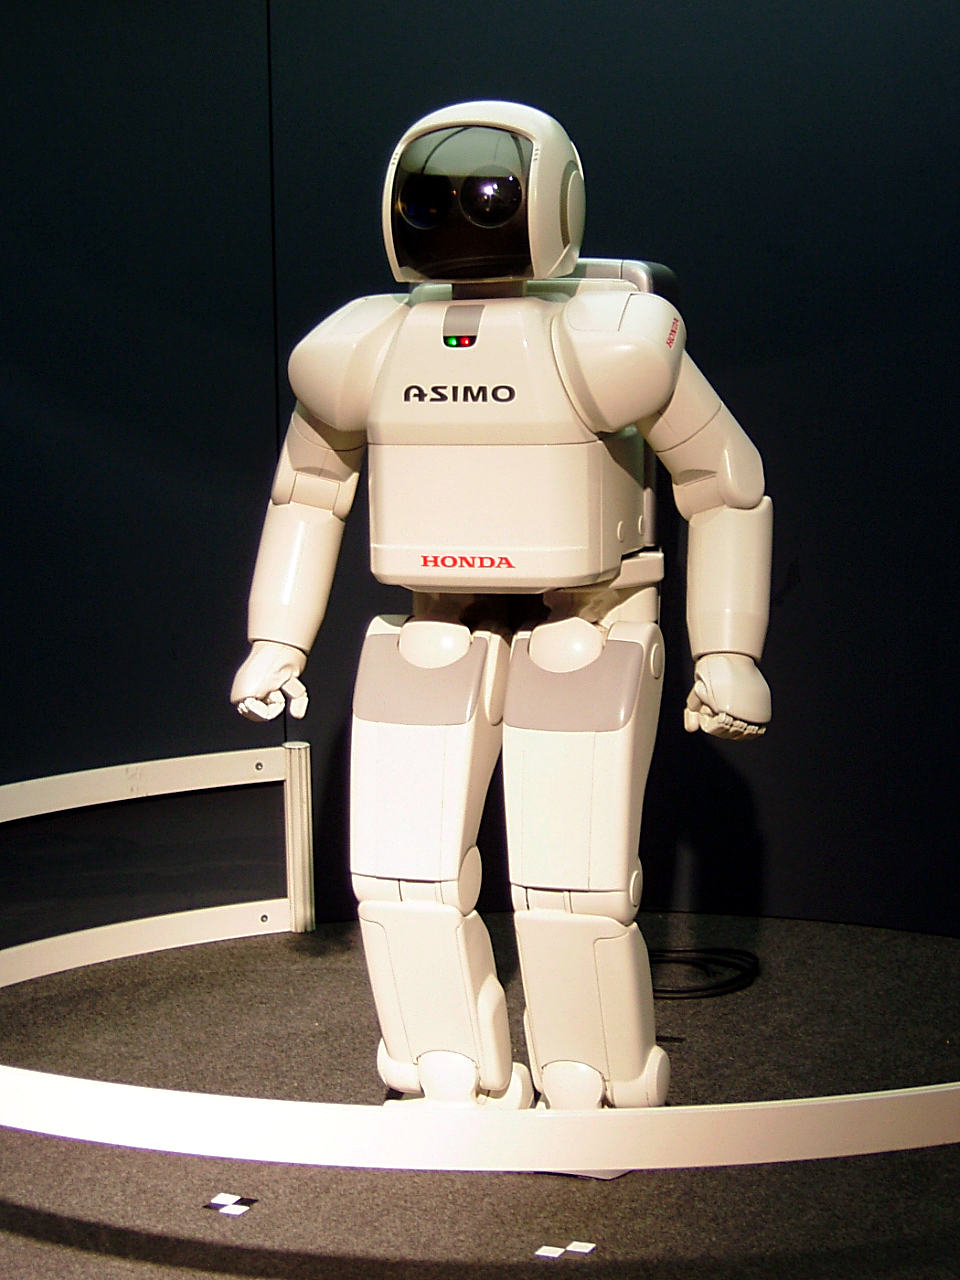
\includegraphics[width=7cm]{grafiken/HONDA_ASIMO.jpg}
\end{minipage}
\begin{minipage}[hbt]{6.7cm}
	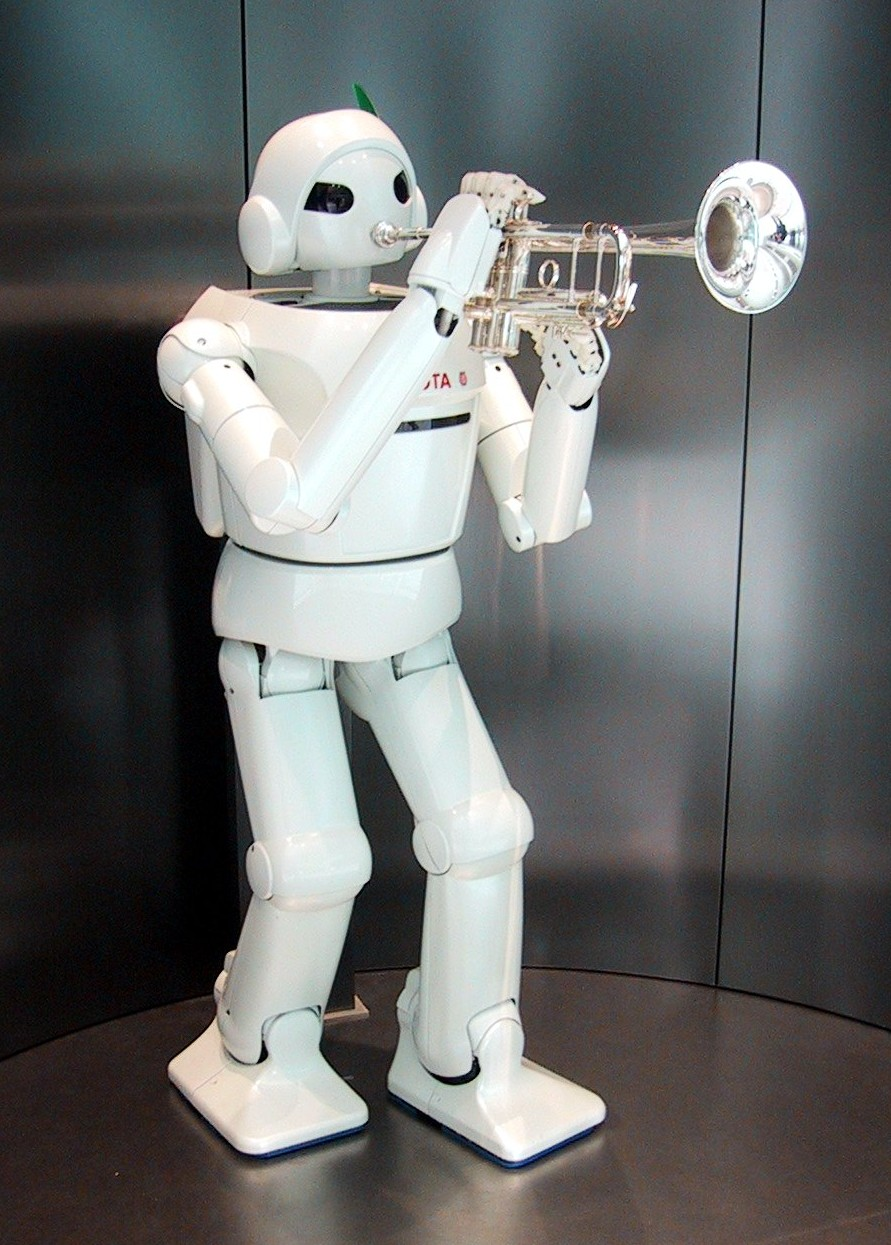
\includegraphics[width=6.7cm]{grafiken/Toyota_Robot_at_Toyota_Kaikan.jpg}
	\end{minipage}
	\caption[Humanoide Roboter]{Humanoide Roboter Links der Aibo von Honda rechts der Roboter von Toyota}
	\label{Humanoide Roboter}
\end{figure}

figure source:(\url{http://de.wikipedia.org/wiki/Humanoider_Roboter})\\Sichtung: 17.09.2010\\\\

In Abb. 1.2 sind...Text\\\\
 
%�bersichtshalber besser Begriffe betonen
Kraft \textbf{F}, der Masse \textbf{m} und der Beschleunigung \textbf{a} kann mit der daraus resultieren Formel die Kraft, die wirkt, berechnet werden: \begin{equation}F = m * a \end{equation} Folglich ist die Kraft das Produkt von Masse und Beschleunigung.  

%Formeln 
SI-Einheit der Kraft:
\begin{equation}
[F] = kg * \frac{m}{s^{2}} = Newton (N)
\end{equation}

\begin{equation}M = F * l = F * r * \sin\alpha \end{equation}
 
SI-Einheit des Drehmomentes: \begin{equation}[M] = Newtonmeter (N * m)\end{equation}
 